\documentclass[10pt,a4paper,twocolumn]{article}
\usepackage[english]{babel}
\usepackage[utf8]{inputenc}
\usepackage[plainpages=false,pdfpagelabels,unicode]{hyperref}
\usepackage[pdftex]{graphicx}
\usepackage[margin=1.5cm, includefoot]{geometry}
\usepackage{authblk}
\usepackage[numbers,sort&compress]{natbib}
\usepackage{mhchem}
\usepackage{multirow}

\author[a,b]{Pavel Ondračka}
\author[c]{David Holec}
\author[a,b]{David Nečas}
\author[a,b]{Lenka Zajíčková}
\affil[a]{Faculty of Science, Masaryk University, Kotlářská 2, 611 37 Brno, Czech Republic}
\affil[b]{CEITEC - Central European Institute of Technology, Masaryk University, Kotlářská 2, 611 37 Brno, Czech Republic}
\affil[c]{Department of Physical Metallurgy and Materials Testing, Montanuniversität Leoben, Franz-Josef-Straße 18, Leoben A-8700, Austria}

% \title{Optical properties of monoclinic, cubic, tetragonal and amorphous HfO$_2$ with TB-mBJ}
\title{Accurate prediction of band gaps and optical properties of HfO$_2$}
\date{}

\begin{document}

\twocolumn[
  \begin{@twocolumnfalse}
    \maketitle
    \begin{abstract}

    \end{abstract}
  \end{@twocolumnfalse}
]

\section{Introduction}
Hafnium dioxide (hafnia, HfO$_2$) is attracting a lot of attention as a perspective high-$k$ material for electronic~\cite{Houssa2006, Robertson2006} as well as optical applications such as antireflective coatings~\cite{Fadel1998, Khoshman2008}, or heat~\cite{Al-Kuhaili2004} and laser mirrors~\cite{Meng2012}.
% Depending on growth conditions, HfO$_2$ has been reported to exist in several polymorhps.
According to an ambient pressure phase diagram, three crystalline polymorphs of \ce{HfO2} are stable (Fig.~\ref{structs}). Namely, a monoclinic structure ($P12_1/c1$, spacegroup: \#14) is stable up to $\sim$1700\,$^\circ$C, a tetragonal phase ($P4_2/nmc$, spacegroup: \#137) appears for temperatures between $\sim$1700\,$^\circ$C and $\sim$2220\,$^\circ$C, while for higher temperatures up to the melting point at $\sim2810\,^{\circ}$C, \ce{HfO2} transforms to a cubic structure ($Fm\bar3m$, spacegroup: \#225)~\cite{Villars2014-px}.

\begin{figure}[b]
   \begin{center}
   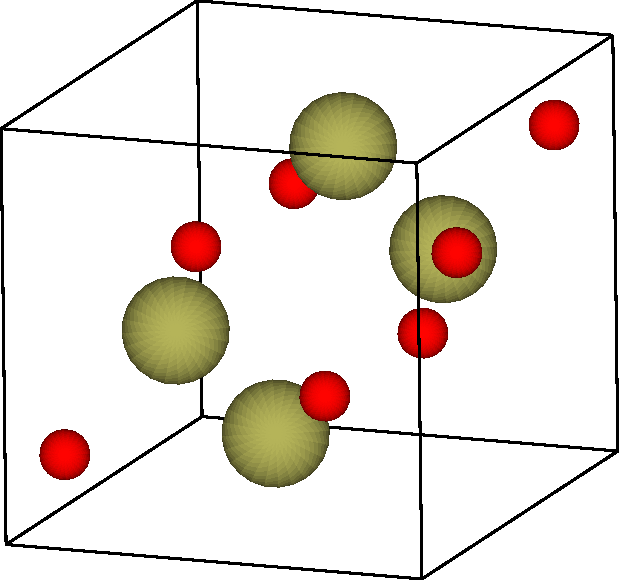
\includegraphics[width=0.3\linewidth]{figures/monoclinic.pdf}
   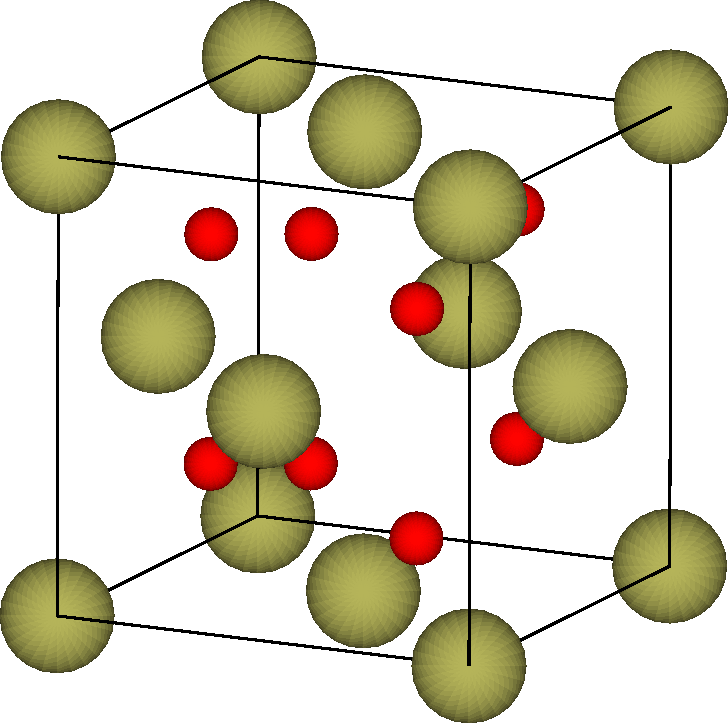
\includegraphics[width=0.3\linewidth]{figures/tetragonal.pdf}
   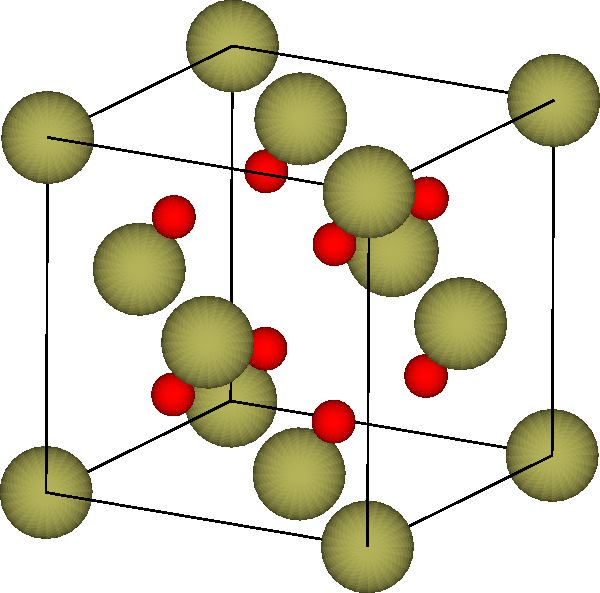
\includegraphics[width=0.3\linewidth]{figures/cubic.pdf}
   \caption{Crystal structure of a) monoclinic, b) tetragonal, and c) cubic hafnia, visualised by VESTA~\cite{Momma2011}.}
   \label{structs}
   \end{center}
\end{figure}

In addition to experimental works, there are numerous modelling, and in particular \textit{ab initio} studies reporting on structural, mechanical, electronic or optical properties of HfO$_2$ \cite{Caravaca2005, Broqvist2007, Ceresoli2006, Garcia2004, Kaneta2007, Liu2009, Scopel2008, Terki2008, Zhao2002, Gruning2010}.
Most of them employ conventional approximations for the exchange-correlation (xc) potential, local density approximation (LDA) or generalised gradient approximation (GGA).
A well known shortcoming of LDA and GGA is an underestimation for the band gap~\cite{Tran2009,Koller2011-hd,Koller2012}.

In order to predict band gaps in much better agreement with experiments, hybrid xc-functionals or other more complex methods (e.g., Green's functions-based GW approach) have been developed, however these are much more computationally expansive in comparison with simple LDA and GGA.
To overcome this difficulty, \citet{Tran2009} have proposed a semi-local xc potential (modified Becke-Johnson, TB-mBJ) that can provide highly accurate band gaps at the computational cost of LDA or GGA.

Using the original TB-mBJ parametrisation, \citet{Koller2012} calculated the and gap of monoclinic HfO$_2$ to be 5.83\,eV , which is in good agreement with the experimental value of 5.68\,eV \cite{Balog1977}.
It is however unclear, whether the predictive power of TB-mBJ for band gaps extends also to other forms of HfO$_2$.
Additionally, since \ce{HfO2} is valued for its optical properties, it is also important to test whether the electronic structure calculated with TB-mBJ xc-potential and yielding improved band gap will guarantee reliable prediction of dielectric function.

Therefore, in this work we critically assess the band gaps and optical properties of monoclinic, tetragonal, cubic and amorphous hafnia calculated with the TB-mBJ potential.

\section{Methodology}

The initial HfO$_2$ monoclinic, tetragonal and cubic cells were structurally optimized with respect to internal positions and lattice parameters.
This was done using the the Vienna Ab initio Simulation Package~\cite{Kresse1996}, with projector augmented pseudopotentials \cite{Kresse1999} and using both, GGA parametrized by Perdew, Burke and Ernzerhof (GGA-PBE) \cite{Perdew1996} as well LDA for the xc-potential.
This is a consequence of a fact, that there is no exchange energy functional associated with the TB-mBJ potential~\cite{Tran2009}, hence its not suitable for structural optimizations based on the total energy minimisation.
The number of $k$-points reflected the size of the modelled cell by keeping product (number of $k$-points)$\cdot$(number of atoms) constant and equal to approximately 2500.
The plane wave cut-off energy of 500\,eV used for crystalline polymorphs was reduced to 300\,eV for the amorphous models.
Consequently, a total energy accuracy of several meV/atom was achieved.

Two amorphous unit cells were prepared by the simulated annealing procedure~[citation needed?].
96 atoms were randomly distributed inside a cubic simulation box with a side 10.1503\,\AA{} corresponding to mass density of 10.695\,g/cm$^3$.
An \textit{ab initio} molecular dynamics run at 5000\,K for 3\,ps with a time step of 3\,fs provided a thermally equilibrated distribution of the atoms inside the cell.
In the next step, the cell temperature was decreased to 0\,K in 100 (fast) or 1000 (slow) steps, each corresponding to 3\,fs.
Finally, the resulting models were structurally relaxed with respect to atom positions and cell volume (i.e., mass density).

Electronic and optical properties were calculated for the structurally optimised models using Wien2k, a full potential all electron code~\cite{Blaha2001} employing the linearized augmented plane wave method.
Dense $k$-grids of 17$\times$17$\times$16 for monoclinic, 24$\times$24$\times$16 for tetragonal, 27$\times$27$\times$27 for cubic, and 4$\times$4$\times$4 for amorphous structures were used in order to obtain converged optical properties.
Atomic spheres radii were set to almost matching spheres corresponding to approximately (depending on polymorph) $\sim$1.7\,\AA{} for oxygen and $\sim$1.9\,\AA{} for hafnium.
The $R_{mt} \cdot K_{max}$ matrix size parameter was set to 9, roughly equivalent to 410\,eV plane wave cut-off energy.

The TB-mBJ with the original parametrisation by \citet{Tran2009} was used for the exchange part, and LDA for the correlation part of the xc-potential. Dielectric functions we calculated using the optic code~\cite{AmbroschDraxl2006}, a part of the Wien2k package, which utilizes Random Phase Approximation (RPA) neglecting local field effects.
A Lorentz broadening of 0.03\,eV was applied to the dielectric function for a better comparison with room temperature experimental data.

\section{Results and discussion}

\subsection{Structural properties}


% FIXME ty tabulky by bylo dobre nejak zkraslit
\begin{table*}
\begin{center}
\caption{Overview of calculated structural properties of monoclinic (m, m2), tetragonal (t), cubic (c) and amorphous (am) phases. $a$, $b$, $c$ are unit cell lattice parameters, $\beta$ is the monoclinic angle, $B$ is bulk modulus, $E_f$ is the energy of formation and $\Delta E_f$ is the difference between $E_f$ for a given phase and the monoclinic (m) phase (the lowest energy configuration). $\rho$ is the mass density.}
\label{structure}
\begin{tabular}{cccccccccc}

\hline
 & & $a$\,[\AA] & $b$\,[\AA] & $c$\,[\AA] & $\beta\,[^{\circ}]$ & $\rho\,[\mathrm{g/cm^3}]$ & $B$\,[GPa] & $E_f$\,[eV/atom] & $\Delta E$\,[eV/atom]\\
\hline\hline

m & GGA & 5.143 & 5.190 & 5.330 & 99.6 & 9.615 & 197 & -3.975 & 0.000
\\%-10.2026 \\
  & LDA & 5.035 & 5.123 & 5.198 & 99.6 & 10.203 & 194 & -4.318 & 0.000
\\%-11.0841 \\
  & exp~\cite{Adam1959} & 5.1156 & 5.1722 & 5.2948 & 99.23 & 9.754 & & & \\
\hline

m2 & GGA & 5.661 & 5.662 & 5.999 & 117.8 & 7.930 & 183 & -3.972 &
0.003\\ %-10.2005 \\
   & LDA & 5.534 & 5.606 & 5.775 & 115.8 & 8.362 & 193 & -4.234 &
0.084\\ %-10.9998 \\
\hline

t & GGA & 3.591 & & 5.219 & 90 & 10.021 & 175 & -3.920 & 0.055\\ %-10.1483 \\
  & LDA & 3.526 & & 5.073 & 90 & 10.693 & 220 & -4.280 & 0.038\\ %-11.0459 \\
  & exp~\cite{Curtis1954} & 5.14 & & 5.25 & & 9.722 & & & \\
\hline

c & GGA & 5.075 & & & 90.0 & 10.318 & 255 & -3.890 & 0.085 \\%-10.1176 \\
  & LDA & 4.982 & & & 90.0 & 10.908 & 289 & -4.261 & 0.057 \\%-11.0274
  & exp~\cite{Senft1983} & 5.110 & 10.109 & & & & & & \\
\hline

%% GGA: Hf: -9.8322 eV/at, O -4.42597 eV/at

am & GGA, slow cooling & & & & & \input{figures/rho-slow.txt} & FIXME & FIXME & FIXME\\ %-10.0043
am & GGA, fast cooling & & & & & \input{figures/rho-fast.txt} & FIXME & FIXME & FIYME\\ %-10.0043
\hline

\end{tabular}
\end{center}
\end{table*}

The four structures considered in the present work (monoclinic, cubic, tetragonal, and amorphous) were fully optimised with respect to the unit cell shape and atom positions at several fixed volumes.
In doing so, we used both GGA and LDA exchange-correlation potentials which typically overestimate and underestimate, respectively, lattice parameters with respect to experimental values.
The thus obtained energy vs. volume data were fitted with Birch-Murnaghan equation of state~\cite{Birch1947}.
Resulting lattice parameters are listed in Table~\ref{structure} together with the selected experimental data from literature for comparison.
The energy of formation was calculated as
\begin{equation}
  E_f^\alpha=E_0(\ce{HfO2}^\alpha) - \frac13 (E_0(\ce{Hf}) + E_0(\ce{O2}))\ ,
\end{equation}
where $E_0(\ce{HfO2}^\alpha)$, $E_0(\ce{Hf})$, and $E_0(\ce{O2})$ are the \textit{ab initio} total energies (per atom) of \ce{HfO2} in the $\alpha$ structure (monoclinic, cubic, tetragonal, or amorphous), Hf in the hcp structure, and an oxygen molecule, respectively.

The most stable structure is, in agreement with the equilibrium phase diagram~\cite{Villars2014-px}, the monoclinic structure, followed by tetragonal (experimentally high temperature) and cubic structures.
The least stable configuration yielding the highest energy of formation, is the amorphous structure.
The optimised lattice parameters are in good agreement with the previously published data, the GGA values being generally closer to the experimental values, hence only the GGA optimised structures were subsequently used in the TB-mBJ calculations.
% QUESTION: Why then TB-mBJ uses LDA and not GGA for the exchange part?
% PAVEL: Actually this is not clear from the original article, however since mBJ is basically empirical based on calibration done with LDA for exchange, I don't thing using it with GGA is a good idea.
% I'll try to clarify this at the mailing list.
The optimisation of the amorphous structure yielded estimates for the equilibrium mass density: $\rho_{\mathrm{slow}}=\input{figures/rho-slow.txt}\,\mathrm{g/cm^3}$, $\rho_{\mathrm{fast}}=\input{figures/rho-fast.txt}\,\mathrm{g/cm^3}$.
These values are slightly lower than for the optimised monoclinic structure (shown in table \ref{structure}), while the tetragonal and cubic structures are also predicted to be more dense.

An interesting phenomenon is predicted for the monoclinic variant.
As shown in Fig.\ref{EV}, the energy vs. volume data exhibit a second minimum (quite a shallow one in the LDA case) for volumes larger than the equilibrium (structural parameters are denoted as m2 in Table~\ref{structure}).
Consequently, a structural transformation is predicted for large isothermal volume expansions.
The most distinct feature is a step-like change of the monoclinic angle $\beta$ from $99.6\,^\circ$ (GGA/LDA) to $117.8\,^\circ$ (GGA) and $115.8\,^\circ$ (LDA) (see bottom panels in Fig.~\ref{EV}).
A similar structural transition has been recently reported for the monoclinic phase in NiTi shape memory alloys \cite{Holec2011-tg}.
There, the structural complexity of the monoclinic phase resulted in a hysteresis of the forwards and backwards pressure-induced phase transformation.
We envision that a similar phenomena may appear also for the monoclinic \ce{HfO2}.

\begin{figure}
\begin{center}
	\includegraphics[width=\linewidth]{figures/m-EV.pdf}
	\caption{Total energy vs. volume data for the monoclinic polymorph calculated with GGA-PBE and LDA. Solid and dashed lines are fits of the Birch-Murnaghan equation of state around the minima m and m2, respectively (only the highlighted points were fitted). The bottom panels show corresponding  monoclinic angle $\beta$ as a function of the volume.}
   \label{EV}
\end{center}
\end{figure}

\subsection{Band gaps}

\begin{table*}
\begin{center}

\caption{Overview of calculated band gaps compared with experimental and other \textit{ab initio} calculations. Band gaps of amorphous structures were obtained using a Tauc plot approach, while the data in brackets are electronic gaps as appearing in, e.g., total density of states (for details see text).}
\label{gaps}

\begin{tabular}{c|cc|ccc}
\hline
& \multicolumn{2}{c|}{present study} & \multicolumn{3}{c}{literature reports}\\
			& TB-mBJ  & PBE & hybrid functionals & GW$_0$ & experiment \\
\hline
\hline
m-HfO$_2$ &	5.76 & 4.08 & PBE0: 6.75~\cite{Komsa2010}, HSE06: 5.98~\cite{Komsa2010} & 5.9~\cite{Gruning2010} & 5.68~\cite{Balog1977} \\
c-HfO$_2$ &	5.88 & 3.77 & SX: 5.6~\cite{Clark2010}, HSE06: 5.38~\cite{Yang2014} & 5.5~\cite{Gruning2010} & 5.8$^A$~\cite{Lim2002}\\
t-HfO$_2$ &	6.54 & 4.79 &  & 6.0~\cite{Gruning2010} & \\
am-HfO$_{2,\mathrm{slow}}$ & 5.47 (5.45) & & \multirow{2}{*}{PBE0: 5.3~\cite{Broqvist2007}, 5.94~\cite{Chen2011}} &  & \multirow{2}{*}{5.49--5.72~\cite{Takeuchi2004}, 5.62~\cite{Nguyen2005}, 5.7~\cite{Perevalov2007}}\\
am-HfO$_{2,\mathrm{fast}}$ & 5.22 (4.78) & &  &  & \\
\hline

\end{tabular}
\end{center}
\end{table*}

The here predicted band gaps for different HfO$_2$ structures are summarised in Table~\ref{gaps} together with experiment data and band gaps calculated using other \textit{ab initio} methods.
A value of 5.76\,eV is obtained for the band gap of m-HfO$_2$ which is perfect agreement with the experimental value of 5.68\,eV~\cite{Balog1977}, and comparable to predictions employing the HSE06 hybrid xc-potential (5.98\,eV)~\cite{Komsa2010} or the GW$_0$ method (5.9\,eV)~\cite{Gruning2010}.
The TB-mBJ value is also in significantly closer to experiment than 6.75\,eV predicted by the PBE0 hybrid functional~\cite{Komsa2010}, and 4.08\,eV obtained from the standard GGA.

The band gap of c-HfO$_2$ was estimated to 5.88\,eV, which is a slightly higher value in comparison with hybrid functionals (SX: 5.6\,eV~\cite{Clark2010}, HSE06: 5.38\,eV~\cite{Yang2014}) as well as the GW$_0$ method (5.5\,eV)~\cite{Gruning2010}.
Comparison with experiment is not straightforward since cubic hafnia is not stable at the room temperature, and hence it is usually stabilized by yttrium.
The band gap of 5.8\,eV~\cite{Lim2002} was reported for (Y$_2$O$_3$)$_{0.15}$(HfO$_2$)$_{0.85}$, which again comparable to our predictions.
It is worth noting, that while for the PBE calculations the band gap for c-HfO$_2$ is 0.3\,eV smaller than that for m-HfO$_2$, the TB-mBJ potential predicts it to be 0.1\,eV larger. 
It thus follows, that the corrections induced by the TB-mBJ xc-potential depend both on the chemistry as well as structural properties.

The largest band gap of all the hafnia polymorphs, is 6.54\,eV, is predicted for the tetragonal structure. 
This is in agreement with the GW$_0$-based calculations, where the band gap of 6.0\,eV is also larger than that of monoclinic and cubic structures, albeit the difference is smaller.
Finally, all TB-mBJ calculated band gaps are significantly increased and improved towards experimental values in comparison with the GGA-PBE values of 4.08, 3.77, and 4.79\,eV for monoclinic, cubic and tetragonal \ce{HfO2}, respectively.

While for the crystalline hafnia structures, the optical band gap was determined directly from the calculations, another approach was chosen for the amorphous cells.
This was necessary in order to achieve a value consistent with experimental measurements, which is traditionally obtained by extrapolating the linear part of $\sqrt{\alpha E n}$ near absorption onset (i.e.so called Tauc plot), where $\alpha$ is the absorption coefficient, $E$ is energy and $n$ is refractive index. %% FIXME Add a reference here!!!
The optical band gap of amorphous cells was estimated by an equivalent approach, i.e., fitting linear part of $\sqrt{J(E)}$ where $J(E)$ is the joint density of states.
% FIXME Should _joint_ dentsity of states be a variable of two energies J(E_1, E_2)???? Maybe some more detailed description will be benefitial here.
% FIXME Could you (or Yeti) provide more justification for this approach (incl. references)?

The two band gap values given in Table~\ref{gaps} correspond to the optical band gap value obtained by aforementioned fitting approach while the value in brackets is the electronic band gap (i.e., the difference between the energy of highest occupied and the lowest unoccupied state).
% FIXME: update gap and optical constants for both am1 and am2 structures when calculations finish.
Calculated optical band gap for amorphous hafnia is 5.65\,eV, again in good agreement with experimental values ranging from 5.49\,eV to 5.72\,eV~\cite{Takeuchi2004, Nguyen2005, Perevalov2007}.
It can be concluded that in case of slow cooling, the effect of defect states on band gap is negligible, in contrast to the fast cooled amorphous cell. We attribute it to the fact that more structural features (resulting in the defect electronic levels) corresponding to the high-temperature amorphous mixture were from ``frozen in'' during the fast cooling process.
% FIXME: does the below sentense make sense?
This may also explain the large spread of the reported experimental values.

\begin{figure}
\begin{center}
	\includegraphics[width=\linewidth]{figures/JDOS.pdf}
	\caption{Tauc-like plot of $\sqrt{J(E)}$ used to estimate optical band gap of the two structural models for amorphous structures. The vertical solid lines denote the data range used for the fitting procedure.}
   \label{JDOS}
\end{center}
\end{figure}

\subsection{Optical properties}

Calculated optical properties are represented by the imaginary part of the dielectric function, $\varepsilon_i$, shown in shown in figures \ref{eps-cHfO2}--\ref{eps-amHfO2} for the 4 here discussed structural modifications of \ce{HfO2}.
The respective crystal symmetry implies that there is one independent component of the dielectric tensor for the cubic structure, two for the tetragonal, and four for the monoclinic hafnia.
Amorphous hafnia was treated as a crystal with only a primitive symmetry (i.e. identity). 
Hence, three diagonal components were calculated, however they were found to be almost identical, and thus confirming the cell amorphousness.
The dielectric tensor is oriented so that the xx component is parallel to the $a$ lattice vector, yy lies in the plane defined by $a$ and $b$ unit cell vectors and is orthogonal to the xx component, and the zz component is perpendicular to the xx and yy components.

Where available, experimental data from literature were added to Figs.~\ref{eps-cHfO2}--\ref{eps-amHfO2} for comparison. 
Despite the qualitative agreement is acceptable, there are some severe qualitative differences.
For example, the calculated imaginary part of $\varepsilon$ for m-HfO$_2$ (Fig.~\ref{eps-mHfO2}b) is underestimated with respect to both experimental dataset by \citet{Edwards2003} and \citet{Nguyen2005}.
% FIXME: Why is it underestimated????
Another obvious disagreement is the failure to reproduce is the peak at 6\,eV appearing in experimental $\varepsilon_i$ of m-\ce{HfO2}.
However, according to \citet{Takeuchi2004}, it originates from oxygen vacancies, and hence its absence in predictions for perfect structures is expected.
Finally, the experiment data seem to exhibit the absorption edge for somewhat lower energies than the predicted $\varepsilon_i$.
% No experimental data are available for tetragonal hafnia.
Similar issues appear when comparing calculated optical properties for cubic and amorphous HfO$_2$ to the measurements of \citet{Lim2002} and \citet{Nguyen2005}, respectively.

To understand better the reason for the above highlighted discrepancies, we have calculated the dielectric function for m-HfO$_2$ also using the hybrid xc-potential, in particular using the Yukawa screened PBE0 functional (YS-PBE0) \cite{Tran2011}.
% FIXME: Why not to add this into Fig. 6 for e.g. one component?
Nevertheless, the spectral dependence remained the same, i.e., also the YS-PBE0-based dielectric function exhibits shift towards higher energies.
% FIXME: I think Yeti was able to interpret this shift, what is its origin. Can you please check it with him?
Therefore we believe that the discrepancy between predicted and experimental data is not caused by inaccurate band structure resulting from the TB-mBJ xc-potential, but rather is cased by the random phase approximation used to calculate the dielectric function.
% FIXME: Can you confirm this by e.g. the BSE calculation? Do you have any data on this? (Just asking, not necessarily to be included in the paper)

%FIXME: 
% Pavel: show the real part or only the imaginary? Maybe some discussion about electronic part of static dielectric constant.
% David: I leave the decision up to you, but I would keep it consistent (Figs. 4-6 have two panels, Fig. 7 only one)!

% FIXME: What is the difference between a) and b)? Is that Re and Im? In such case, I think the label should be only epsilon, not epsilon_i??? Or it should be epsilon_r in a) and epsilon_i in b)???

% FIXME: It would be good to use always the same style (colour, type of line) for the experimental data, to help the reader.

\begin{figure}
\begin{center}
	\includegraphics[width=\linewidth]{figures/c-HfO2.pdf}
	\caption{Calculated dielectric function of c-HfO$_2$}
   \label{eps-cHfO2}
\end{center}
\end{figure}

\begin{figure}
\begin{center}
	\includegraphics[width=\linewidth]{figures/t-HfO2.pdf}
	\caption{Calculated dielectric function of t-HfO$_2$}
   \label{eps-tHfO2}
\end{center}
\end{figure}

\begin{figure}
\begin{center}
% FIXME: This is confusing: dash-dot purple line is calc epsilon_1_xz in a) while it is exp in b)!!!!
	\includegraphics[width=\linewidth]{figures/m-HfO2.pdf}
	\caption{Calculated dielectric function of m-HfO$_2$}
   \label{eps-mHfO2}
\end{center}
\end{figure}

\begin{figure}
\begin{center}
	\includegraphics[width=\linewidth]{figures/am-HfO2.pdf}
	\caption{Calculated dielectric function of am-HfO$_2$}
   \label{eps-amHfO2}
\end{center}
\end{figure}


\section{Conclusions}

In this work, we have thoroughly tested the performance of the TB-mBJ exchange-correlation potential for predicting optical band gaps and dielectric function of several \ce{HfO2} polymorhps.
These include crystalline monoclinic, tetragonal and cubic phases as appearing in the equilibrium phase diagram, and were complemented by a supercell model for amorphous structure which is often obtained experimentally due to specific growth conditions.
% All models were optimized with respect to the latice parameters and atomic positions using the standard LDA and GGA-PBE exchange-correlation potentials.
% Then band gaps and optical properties were calculated using TB-mBJ.
The predicted band gaps were found in excellent agreement with available experimental data, as well as with (or sometimes even better than) the previously reported valued calculated by much more computationally expansive hybrid or GW approaches.
Despite a reasonable qualitative agreement, the calculated dielectric functions for all polymorhps exhibit a shift of their spectral weights to higher energies with respect to experiment data.
This was attributed to approximations used during the calculation of the optical properties (e.g., random phase approximation and omission of local field effects) rather than deficiencies in the calculated band structure.
  
\section*{Acknowledgments}
This work was supported by the IT4Innovations Centre of Excellence project (CZ.1.05/1.1.00/02.0070), funded by the European Regional Development Fund and the national budget of the Czech Republic via the Research and Development for Innovations Operational Programme, as well as Czech Ministry of Education, Youth and Sports via the project Large Research, Development and Innovations Infrastructures (LM2011033).
% FIXME: acknowledgments for CEITEC and probably MOBILITY?

\bibliographystyle{unsrtnat}
\bibliography{bib-db}

\end{document}
